
%% bare_conf.tex
%% V1.3
%% 2007/01/11
%% by Michael Shell
%% See:
%% http://www.michaelshell.org/
%% for current contact information.
%%
%% This is a skeleton file demonstrating the use of IEEEtran.cls
%% (requires IEEEtran.cls version 1.7 or later) with an IEEE conference paper.
%%
%% Support sites:
%% http://www.michaelshell.org/tex/ieeetran/
%% http://www.ctan.org/tex-archive/macros/latex/contrib/IEEEtran/
%% and
%% http://www.ieee.org/

%%*************************************************************************
%% Legal Notice:
%% This code is offered as-is without any warranty either expressed or
%% implied; without even the implied warranty of MERCHANTABILITY or
%% FITNESS FOR A PARTICULAR PURPOSE! 
%% User assumes all risk.
%% In no event shall IEEE or any contributor to this code be liable for
%% any damages or losses, including, but not limited to, incidental,
%% consequential, or any other damages, resulting from the use or misuse
%% of any information contained here.
%%
%% All comments are the opinions of their respective authors and are not
%% necessarily endorsed by the IEEE.
%%
%% This work is distributed under the LaTeX Project Public License (LPPL)
%% ( http://www.latex-project.org/ ) version 1.3, and may be freely used,
%% distributed and modified. A copy of the LPPL, version 1.3, is included
%% in the base LaTeX documentation of all distributions of LaTeX released
%% 2003/12/01 or later.
%% Retain all contribution notices and credits.
%% ** Modified files should be clearly indicated as such, including  **
%% ** renaming them and changing author support contact information. **
%%
%% File list of work: IEEEtran.cls, IEEEtran_HOWTO.pdf, bare_adv.tex,
%%                    bare_conf.tex, bare_jrnl.tex, bare_jrnl_compsoc.tex
%%*************************************************************************

% *** Authors should verify (and, if needed, correct) their LaTeX system  ***
% *** with the testflow diagnostic prior to trusting their LaTeX platform ***
% *** with production work. IEEE's font choices can trigger bugs that do  ***
% *** not appear when using other class files.                            ***
% The testflow support page is at:
% http://www.michaelshell.org/tex/testflow/



% Note that the a4paper option is mainly intended so that authors in
% countries using A4 can easily print to A4 and see how their papers will
% look in print - the typesetting of the document will not typically be
% affected with changes in paper size (but the bottom and side margins will).
% Use the testflow package mentioned above to verify correct handling of
% both paper sizes by the user's LaTeX system.
%
% Also note that the "draftcls" or "draftclsnofoot", not "draft", option
% should be used if it is desired that the figures are to be displayed in
% draft mode.
%
\documentclass[10pt, conference, compsocconf]{IEEEtran}
% Add the compsocconf option for Computer Society conferences.
%
% If IEEEtran.cls has not been installed into the LaTeX system files,
% manually specify the path to it like:
% \documentclass[conference]{../sty/IEEEtran}





% Some very useful LaTeX packages include:
% (uncomment the ones you want to load)


% *** MISC UTILITY PACKAGES ***
%
%\usepackage{ifpdf}
% Heiko Oberdiek's ifpdf.sty is very useful if you need conditional
% compilation based on whether the output is pdf or dvi.
% usage:
% \ifpdf
%   % pdf code
% \else
%   % dvi code
% \fi
% The latest version of ifpdf.sty can be obtained from:
% http://www.ctan.org/tex-archive/macros/latex/contrib/oberdiek/
% Also, note that IEEEtran.cls V1.7 and later provides a builtin
% \ifCLASSINFOpdf conditional that works the same way.
% When switching from latex to pdflatex and vice-versa, the compiler may
% have to be run twice to clear warning/error messages.






% *** CITATION PACKAGES ***
%
%\usepackage{cite}
% cite.sty was written by Donald Arseneau
% V1.6 and later of IEEEtran pre-defines the format of the cite.sty package
% \cite{} output to follow that of IEEE. Loading the cite package will
% result in citation numbers being automatically sorted and properly
% "compressed/ranged". e.g., [1], [9], [2], [7], [5], [6] without using
% cite.sty will become [1], [2], [5]--[7], [9] using cite.sty. cite.sty's
% \cite will automatically add leading space, if needed. Use cite.sty's
% noadjust option (cite.sty V3.8 and later) if you want to turn this off.
% cite.sty is already installed on most LaTeX systems. Be sure and use
% version 4.0 (2003-05-27) and later if using hyperref.sty. cite.sty does
% not currently provide for hyperlinked citations.
% The latest version can be obtained at:
% http://www.ctan.org/tex-archive/macros/latex/contrib/cite/
% The documentation is contained in the cite.sty file itself.






% *** GRAPHICS RELATED PACKAGES ***
%
\ifCLASSINFOpdf
  % \usepackage[pdftex]{graphicx}
  % declare the path(s) where your graphic files are
  % \graphicspath{{../pdf/}{../jpeg/}}
  % and their extensions so you won't have to specify these with
  % every instance of \includegraphics
  % \DeclareGraphicsExtensions{.pdf,.jpeg,.png}
\else
  % or other class option (dvipsone, dvipdf, if not using dvips). graphicx
  % will default to the driver specified in the system graphics.cfg if no
  % driver is specified.
  % \usepackage[dvips]{graphicx}
  % declare the path(s) where your graphic files are
  % \graphicspath{{../eps/}}
  % and their extensions so you won't have to specify these with
  % every instance of \includegraphics
  % \DeclareGraphicsExtensions{.eps}
\fi
% graphicx was written by David Carlisle and Sebastian Rahtz. It is
% required if you want graphics, photos, etc. graphicx.sty is already
% installed on most LaTeX systems. The latest version and documentation can
% be obtained at: 
% http://www.ctan.org/tex-archive/macros/latex/required/graphics/
% Another good source of documentation is "Using Imported Graphics in
% LaTeX2e" by Keith Reckdahl which can be found as epslatex.ps or
% epslatex.pdf at: http://www.ctan.org/tex-archive/info/
%
% latex, and pdflatex in dvi mode, support graphics in encapsulated
% postscript (.eps) format. pdflatex in pdf mode supports graphics
% in .pdf, .jpeg, .png and .mps (metapost) formats. Users should ensure
% that all non-photo figures use a vector format (.eps, .pdf, .mps) and
% not a bitmapped formats (.jpeg, .png). IEEE frowns on bitmapped formats
% which can result in "jaggedy"/blurry rendering of lines and letters as
% well as large increases in file sizes.
%
% You can find documentation about the pdfTeX application at:
% http://www.tug.org/applications/pdftex





% *** MATH PACKAGES ***
%
%\usepackage[cmex10]{amsmath}
% A popular package from the American Mathematical Society that provides
% many useful and powerful commands for dealing with mathematics. If using
% it, be sure to load this package with the cmex10 option to ensure that
% only type 1 fonts will utilized at all point sizes. Without this option,
% it is possible that some math symbols, particularly those within
% footnotes, will be rendered in bitmap form which will result in a
% document that can not be IEEE Xplore compliant!
%
% Also, note that the amsmath package sets \interdisplaylinepenalty to 10000
% thus preventing page breaks from occurring within multiline equations. Use:
%\interdisplaylinepenalty=2500
% after loading amsmath to restore such page breaks as IEEEtran.cls normally
% does. amsmath.sty is already installed on most LaTeX systems. The latest
% version and documentation can be obtained at:
% http://www.ctan.org/tex-archive/macros/latex/required/amslatex/math/





% *** SPECIALIZED LIST PACKAGES ***
%
%\usepackage{algorithmic}
% algorithmic.sty was written by Peter Williams and Rogerio Brito.
% This package provides an algorithmic environment fo describing algorithms.
% You can use the algorithmic environment in-text or within a figure
% environment to provide for a floating algorithm. Do NOT use the algorithm
% floating environment provided by algorithm.sty (by the same authors) or
% algorithm2e.sty (by Christophe Fiorio) as IEEE does not use dedicated
% algorithm float types and packages that provide these will not provide
% correct IEEE style captions. The latest version and documentation of
% algorithmic.sty can be obtained at:
% http://www.ctan.org/tex-archive/macros/latex/contrib/algorithms/
% There is also a support site at:
% http://algorithms.berlios.de/index.html
% Also of interest may be the (relatively newer and more customizable)
% algorithmicx.sty package by Szasz Janos:
% http://www.ctan.org/tex-archive/macros/latex/contrib/algorithmicx/






% correct bad hyphenation here
\hyphenation{op-tical net-works semi-conduc-tor}
\usepackage{multirow}
\usepackage{amsmath}
\usepackage{systeme}
\usepackage{graphicx}
\usepackage{subcaption}
\usepackage{caption}

\begin{document}
%
% paper title
% can use linebreaks \\ within to get better formatting as desired
%\title{Quantification of energy savings in smart buildings, physics or data?}

%\title{A novel data driven approach for the quantification of energy savings in smart buildings}
\title{Data driven modelling for energy consumption prediction on smart buildings}
 
 
% author names and affiliations
% use a multiple column layout for up to two different
% affiliations

\author{\IEEEauthorblockN{Aurora Gonz\'alez-Vidal}
\IEEEauthorblockA{Department of Information and Communication Engineering\\
Computer Science\\
University of Murcia, Spain\\
aurora.gonzalez2@um.es}
\and
\IEEEauthorblockN{Alfonso P. Ramallo-Gonz\'alez}
\IEEEauthorblockA{Department of Information and Communication Engineering\\
Computer Science\\
University of Murcia, Spain\\
alfonso.ramallo@um.es}
\and
\IEEEauthorblockN{Fernando Terroso-S\'aenz}
\IEEEauthorblockA{Department of Information and Communication Engineering\\
Computer Science\\
University of Murcia, Spain\\
fterroso@um.es}
\and
\IEEEauthorblockN{Antonio Skarmeta}
\IEEEauthorblockA{Department of Information and Communication Engineering\\
Computer Science\\
University of Murcia, Spain\\
skarmeta@um.es}

}

% conference papers do not typically use \thanks and this command
% is locked out in conference mode. If really needed, such as for
% the acknowledgment of grants, issue a \IEEEoverridecommandlockouts
% after \documentclass

% for over three affiliations, or if they all won't fit within the width
% of the page, use this alternative format:
% 
%\author{\IEEEauthorblockN{Michael Shell\IEEEauthorrefmark{1},
%Homer Simpson\IEEEauthorrefmark{2},
%James Kirk\IEEEauthorrefmark{3}, 
%Montgomery Scott\IEEEauthorrefmark{3} and
%Eldon Tyrell\IEEEauthorrefmark{4}}
%\IEEEauthorblockA{\IEEEauthorrefmark{1}School of Electrical and Computer Engineering\\
%Georgia Institute of Technology,
%Atlanta, Georgia 30332--0250\\ Email: see http://www.michaelshell.org/contact.html}
%\IEEEauthorblockA{\IEEEauthorrefmark{2}Twentieth Century Fox, Springfield, USA\\
%Email: homer@thesimpsons.com}
%\IEEEauthorblockA{\IEEEauthorrefmark{3}Starfleet Academy, San Francisco, California 96678-2391\\
%Telephone: (800) 555--1212, Fax: (888) 555--1212}
%\IEEEauthorblockA{\IEEEauthorrefmark{4}Tyrell Inc., 123 Replicant Street, Los Angeles, California 90210--4321}}




% use for special paper notices
%\IEEEspecialpapernotice{(Invited Paper)}




% make the title area
\maketitle


\begin{abstract}

Many efforts from several organisations are focused on increasing energy efficiency. This is on the interest of everybody, from individuals to governments, since energy efficiency yields to economical savings, to reduce greenhouse gas emissions and to alleviate energy poverty. Buildings are one of the largest consumers of primary energy and its efficiency is an important goal for the achievement of the mentioned goals.   % as it contributes to growth and more jobs.

%Before implementing an energy efficiency solution than aims to behavioural changes, it is necessary to define the relationship which exists between energy use and building operating conditions. Knowing that could determine energy savings resulting from the implementation of the solution. 

%White box models based on physical equations have been used to model buildings' systems, and to predict whole buildings and the behaviour of their sub-systems, such as their energy consumption and indoor comfort. However, 
Currently, the new paradigm of the Internet of Things allow us to count on vast amounts of data that can be used for knowledge extraction of all kinds, one can expect that energy prediction will not be an exception.

This new paradigm that brings large amounts of data, and the advantages on machine learning, have motivated us to test the hypothesis of this paper. This hypothesis supports that prior information that one can find on the physics of the building heat transfer, is now redundant due to the completeness of the data from the system.

We propose a machine learning approach and a grey-box model approach to test this hypothesis, the first blind to the physiscs of the problem, and the second heavily influenced by it. The energy consumption prediction models were created with the two approaches. The method has been designed to be used on a project in which the evaluation of energy efficiency interventions is tested. However, the model at this stage was designed to estimate the energy consumption in normal operation state i.e. if the system would not have been altered by any energy efficiency intervention.

%We propose a machine learning approach and a grey-box model approach for the creation of an energy consumption prediction model that is used to estimate the energy consumption in normal operation state, i.e., if the  system would not have been altered by the energy efficiency experiment. %This allows us to compare the predicted for normal operating state and the actual consumption in order to quantify the energy savings.

Our black-box method, which is based on a combination of statistical, machine learning models and on a time series structurisation of the data, shows better prediction accuracy than the so-called grey-box methods that include basic physical equations. This proves for this case that the hypothesis of this paper can be rejected i.e. also in this field a data driven approach outperforms more informed methods.

\end{abstract}

\begin{IEEEkeywords}
data-driven models, black-box models, grey-box models, smart buildings, data analytics

\end{IEEEkeywords}


% For peer review papers, you can put extra information on the cover
% page as needed:
% \ifCLASSOPTIONpeerreview
% \begin{center} \bfseries EDICS Category: 3-BBND \end{center}
% \fi
%
% For peerreview papers, this IEEEtran command inserts a page break and
% creates the second title. It will be ignored for other modes.
\IEEEpeerreviewmaketitle



\section{Introduction} \label{intro}

Energy consumption of buildings in developed countries comprises 20-40\% of their total energy use and it is above industry and transport in EU and US \cite{perez2008review, energyUS}. 

In order to mitigate climate change, the reduction of energy use together with the use of non-fossil energy sources such as solar and wind is crucial. On the other hand, reducing energy consumption on buildings has to be done always maintaining the necessary levels so as to keep comfort for buildings users and to lower their costs to not increase fuel-poverty. Seems like the new sensorisation of buildings might be openning the door for solving these issues.

When it comes to energy savings, energy management should be the process of monitoring, controlling, and conserving energy during buildings' normal use.  The prediction of energy use in buildings is a powerfull piece of information, that is fundamental in concenrs such micro-grids, energy storage, demands analysis or energy feedback. Novel energy feedback systems involve the following steps:

\begin{itemize}
\item Metering and collecting energy consumption data,
\item Proposing ways of saving energy by analysing the data and putting them into practice, and
\item Tracking the consumption in order to quantify the gains due to the proposed activity.
\end{itemize}

%We consider that there is a lack of variety in the way the third step is tackled nowadays. 

The series of methods and processes used to face the third step, that is to asses the performance of energy efficiency interventions by quantifying the gains on efficiency are commonly noted as Evaluation, Measurement, and Verification (EM\&V). 

%In terms of the third step, the gains quantification is done through a collection of methods and processes used to assess the performance of energy efficiency activities called Evaluation, Measurement, and Verification (EM\&V). This has 

%The main objectives of an EM\&V process are to assess the performance of an energy efficiency program or project, to measure the energy or demand savings, and to determine if the program is generating the expected level of savings.

%The traditional EM\&V methods for determine if a program is generating the expected level of savings are based on linear regression models and they are described in the ASHRAE’s Guideline \cite{ashrae2002ashrae}. 
The energy consumption evaluation compared to prior intervention scenarios is currently developing and  simple regression models, such the ones proposed in the ASHRAEs Guideline \cite{ashrae2002ashrae}, might not be enough at this moment. Several researchers are focusing on the development of $EM\&V$  methods with a less naive perspectives \cite{ramalloidentifying}. 



Regression models need to be typically adjusted in an \textit{ad hoc} manner in order to capture non-linear behavior, which arises from complex (physical) multi-variate interactions between ambient conditions, occupancy, building operating conditions and so forth \cite{heo2012gaussian}.

%[Expalin why we choose data analytics]

Regression has always been the standard approach to modelling the relationship between one outcome variable  and several input variables, and it can be seen both from a white-box and a black-box point of view. That means, we could use regression for analytical purposes, where a scenario is understood through physics or for data-driven purposes where a scenario is modeled using data alone. 


In recent years, a new phenomenon is affecting the building sector, and this is the proliferation of smart meters and in home displays, and the trend seems to be on the rise considering that the European Commission has established that 16 Member States will proceed with large-scale roll-out of smart meters by 2020 or earlier \cite{ec2014report}. This together with the new developments on Energy Data Infrastructure (such as \cite{terroso2017open, fotopoulou2017providing}) has formed the perfect growing soil for the creation among other technologies of advanced energy feedback strategies for the reduction of energy use in buildings and for the education of building occupants/users \cite{how2017}. The correct prediction of consumptions is crucial for the functioning of those.

Thanks to that, the generation of data about our surrounding environment and ourselves is explosively growing in terms of \emph{velocity}, \emph{variety} and \emph{volume}. This implies that there is more value hidden in the data than it has never been before and that as the datasets are generally too large for classical methods (with indicators such as p-value) to have meaning. Now, predictive data-driven modelling uses other ways to fit a mosdel such as machine learning, and these approaches are fastly taking over in many disciplines.

%The other way to approach our problem is analytically, where models are often based on our understading of nature through physics. Those are called white-box models.

%https://ibm.cioreview.com/cxoinsight/the--black-box-paradox--in-big-data-analytics-and-datadriven-modelling-nid-18145-cid-117.html

%Analytical models are often based on a human’s understanding of nature, while data-driven and machine learning models attempt to model nature using data alone. Some data-driven models, such as linear regression, are transparent and interpretable, while other “black-box” models are not transparent and can be difficult to interpret.

Our proposal for energy consumption is to take a machine learning approach, where black-box models are used in order to predict energy consumption, reducing the cost compared to traditional white box processes which require a level of building engineering expertise that limits scalability. This has also been compared with a grey-box approach, that lays between the previous two.




%\subsection{Regression vs Machine Learning}

%The Difference Between Predictive modelling and Regression 

%when using predictive modelling, we can use many different models simultaneously, and compare  them to find the one that is the best. We can use the traditional regression, but also decision trees  and neural network analysis. We can also combine  different models. We can focus on accuracy of prediction rather than just i dentifying risk factors

%Regression requires an assumption of normality. The definition of confidence intervals, too, requires normality.

%Additional assumptions for regression are that the mean of the error term is equal to zero, and that the error term has equal variance for different levels of the input or independent variables. While the assumption of  zero mean is almost always satisfied, the assumpti on of equal variance is not

%With recent advances in sensor and communication technologies, the generation of data about our surrounding environment and ourselves is explosively growing in terms of \emph{velocity}, \emph{variety} and \emph{volume} \cite{ali2014}. The treatment of huge data sets challenges traditional technologies and promotes the emergence of \textbf{Big Data} tools in order to capture, store, manage and analyze such data. In this context, \textbf{Internet of Things (IoT)} is one of the key enablers of \textbf{Smart Cities}. We are part of a new \emph{Era} where sensing technologies are being exploited to create innovative services for Citizens and Service Providers.


%[Explain why daily and weekly is our interest]


\section{Related work}

Building thermodynamics is a complex nonlinear phenomenon, which is strongly influenced by weather conditions, building operating modes, and occupant schedules.

Three general categories of building energy forecasting models have been reported in the literature which include white-box (physics-based), black-box (data-driven), and grey-box (combination of physics based and data-driven) modelling approaches \cite{li2014review}.

\subsection{White-box models}


Building structure, systems and equipments need to be considered for this kind of models together with weather and other boundary conditions. The first are usually obtained from design plans, manufacture catalogues or visual inspection.

There exist a wealth of mature white box simulation engines that through the combination of mathematical equations, simulate the building and calculate its energy consumption. Well-known engines such as EnergyPlus \cite{crawley2001energyplus} and TRNSYS \cite{TRNSYS} have been widely used to analyse energy consumption and determine building control and operation schemes among others \cite{crawley2008contrasting}.

Even though these elaborate simulation tools are effective and accurate, they require detailed information and input parameters. These parameters, however, are in most cases difficult to obtain, and sometimes not available.

\subsection{Black-box models}


Black-box models are also known as solely data-driven models. In this case, statistical models are directly applied to capture the relationship between building energy consumption and the inputs such as operation and weather data. This type of models need baseline measurements over a certain period of time.

Regression can be used as a data-driven model. But this method is highly more interpretable than machine learning approaches. 
Machine learning systems figure out how to solve problems with minimal human guidance and once a machine learning algorithm is trained, it can be difficult to understand why it gives a particular response to a set of inputs. 

The adaptability of the machine learning models through the cross-validation process that tunes their hyperparameters (which is different from mathematical models such as regression models) makes accurate decisions without outside expert intervention which comes out useful when unusual perturbations, disturbances, and/or changes in building background conditions may occur.

Several data-based modelling techniques have been used for EM\&V, including multiple linear regression \cite{braun2014using}.  %time series [4], 
In the case of machine learning techniques such as neural networks, support vector machines and their combination \cite{ahmad2014review}, Gaussian Process modelling \cite{heo2012gaussian}, and fuzzy logic models \cite{ciabattoni2014fuzzy} are some examples. In such studies, the way of relating energy consumption and the input variables is instantaneous. That means, the energy consumption is only related to current indicators such as the temperature, humidity and others at a given timestamp.
%for predicting hourly energy consumption the used inputs are taken out of the state of the exact moment that has to be predicted: same hour mean temperature, and so on.
  

\subsection{Grey-box models}

Grey-box models use simplified physical descriptions to simulate the behaviour of building energy systems, and with them identify important parameters and characteristics using statistical analysis \cite{handbook2017american}.
%Both statistical and machine learning methods need sufficient historical data to provide accurate models. 

Data-driven modelling based on grey-box models have been used for many years. As early of 1951 Burnard demonstrated for the first time that resistor-capacitor (RC) networks can represent the thermodynamics of buildings accurately \cite{burnand1952study}. Since then, RC-networks have been used to represent the thermodynamics of buildings. In the early years of building dynamic simulation, this was one of the few ways of representing the thermodynamics of buildings, but even today, programs such as EnergyPlus, include thermal networks on their codes \cite{handbook2017american} .

In addition to building simulation, grey-box modelling of buildings using RC-networks have been used for the last two decades for Model Predictive Control (MC). MC has been used to govern heating and cooling systems of normally large buildings in a way in which the controller can anticipate to the needs of the building via the previous estimation of its thermodynamic features (these normally translated into response times and conductivity of the thermal envelope) \cite{coley1992second}.

This has motivated the investigation of ideal model topologies and methodologies for these models to ensure that they represent accurately the responses of buildings \cite{bacher2011identifying}. But also, other works are now focusing on how those methods can be used for the characterisation of their thermal envelope \cite{ramallo2017reliability}.

In cases where limited amounts of data are available and the information about the building architecture is partially known, grey models are suitable alternatives for the prediction of energy consumption \cite{hamzacebi2014forecasting}.



%A new approach to energy consumption prediction of domestic heat pump water heater based on grey system theory





%Artificial neural networks (ANN) is another popular method in building energy modelling for building operation purpose.

%predict cooling demand in a building. The energy demand was predicted using its measured or predicted values as well as the predicted values of air temperature and relative humidity \cite{yokoyama2009prediction}



\section{Methodology}

In this section we introduce both a black-box model and use a grey-box model in order to estimate the energy consumption of a building.

\subsection{Inputs}


Energy forecasting studies that use machine learning are usually intended to predict consumption \textbf{a priori} in order to manage and store the suitable amount of energy, taking into consideration the market prizes and also the necessities of the buildings. However, our approach is different in the sense that our goal is to quantify the energy savings relative to a baseline period due to certain experiment related to efficiency improvement. 
%evaluate a particular action that has been developed during a period of time and the prediction is done afterwards.

This translates into a difference on the inputs that are available for the prediction. In other scenarios, data concerning energy consumption in previous hours and days is largely useful because it is evidently highly correlated with the later consumption \cite{aman2014empirical}. However, we should not use such data because in case of using this algorithm on a building in which an intervention for energy reduction has taken place the consumption is likely to be altered by the experiment.

On the other side, in other scenarios environmental data is not available yet (it is the future) and predictions have to be used. When applying prediction for EM\&V, environmental and occupation variables are usually available and it is not necessary to predict them. The most commonly used weather information is outdoor dry-bulb air temperature and solar irradiance, but in our case temperature was seen to be sufficient.



\subsection{Proposed models}

Our interest lies on weekly quantification of the energy use. However, daily dynamics are useful since there exist patterns that can be found depending on the day of the week. Our model predicts daily energy consumption and then compute the metrics on an aggregated manner so that the global quantification is done weekly.

Using this data, we then tested three approaches:

\subsubsection{Black-box}

Daily aggregate consumption is used as output and we try to capture the relationship between daily average temperature and the consumption by relating the time series composed by temperature hourly means and the daily consumption.

After this, we used several machine learning models in order to asses which one is the best one for our scenarios. The models are generated  following the next steps \cite{gonzalez2016towards}:

\begin{itemize}
\item Clean and transform the data: selecting predictive variables such as temperature and day type, deleting outliers 
\item Aggregate: compute daily consumption, create the time series with the input variables and represent the series in a lower dimension. That is, apply hourly average or other representation and feature selection methods in order to serve as inputs of our models.
\item Divide the dataset into train (75 \% ) and test (25 \%)
\item Validation method: 10-fold cross validation and 5 repetitions over the training data set in order to find the hyperparameters of each machine learning algorithm
\item Evaluate: apply the algorithm to the test dataset in order to obtain the metric for the model fitting
\end{itemize}


To our knowledge, our method differs from existing methods in the way which the data is introduced. We are relating the input as a time series with a single output. This has been previously done in scenarios in which consumption could be used as a predictor \cite{ruijin2013building}, that means, where the energy consumption is not altered by any intervention and the goal is simply to make a prediction of the energy a priori, with storage and production intentions. However, this is not possible for EM\&V, as it is our case, resulting on a novel application of the method.

We have avoided the use of change-point models adding novelty to our approach. In a vast amount of energy efficiency literature, change-point models are used to determine the outdoor air temperatures at which the building transitions from heating to the dead-band and from the dead-band to cooling (like in \cite{kissock1998ambient}). However, we cover such effect by using the time series of the  daily means of the temperature. 


\subsubsection{ Grey-box}


To make use of this models the set of outputs and inputs have to be defined together with the topology of the system. 
The most common mathematical representation of lumped parameter models is the state-space representation. The general form for time-invariant models can be written as shown on Eq. \ref{eq1}

\begin{equation}\label{eq1}
\systeme*{x'(t)=Ax(t) + Bu(t), y(t)= Cx(t) + Du(t)}
\end{equation}

where $x$ is a vector with the states of the model, in our case the temperatures, $A$ is a characteristic matrix of the model, $B$ defines the effect of the inputs in the model, and $u$ are the inputs, in our case the outside temperature and electric gains. In this formulation, $y$ represents the variables that are measured, in our case electricity. $C$ is the identity matrix; and $D$ is zero in all cases for this work. Using this formulation, every time that a solution had to be evaluated the Octave built in function \textbf{lsim} was used.

\begin{figure}[h]%\vspace*{4pt}
\centering
\centerline{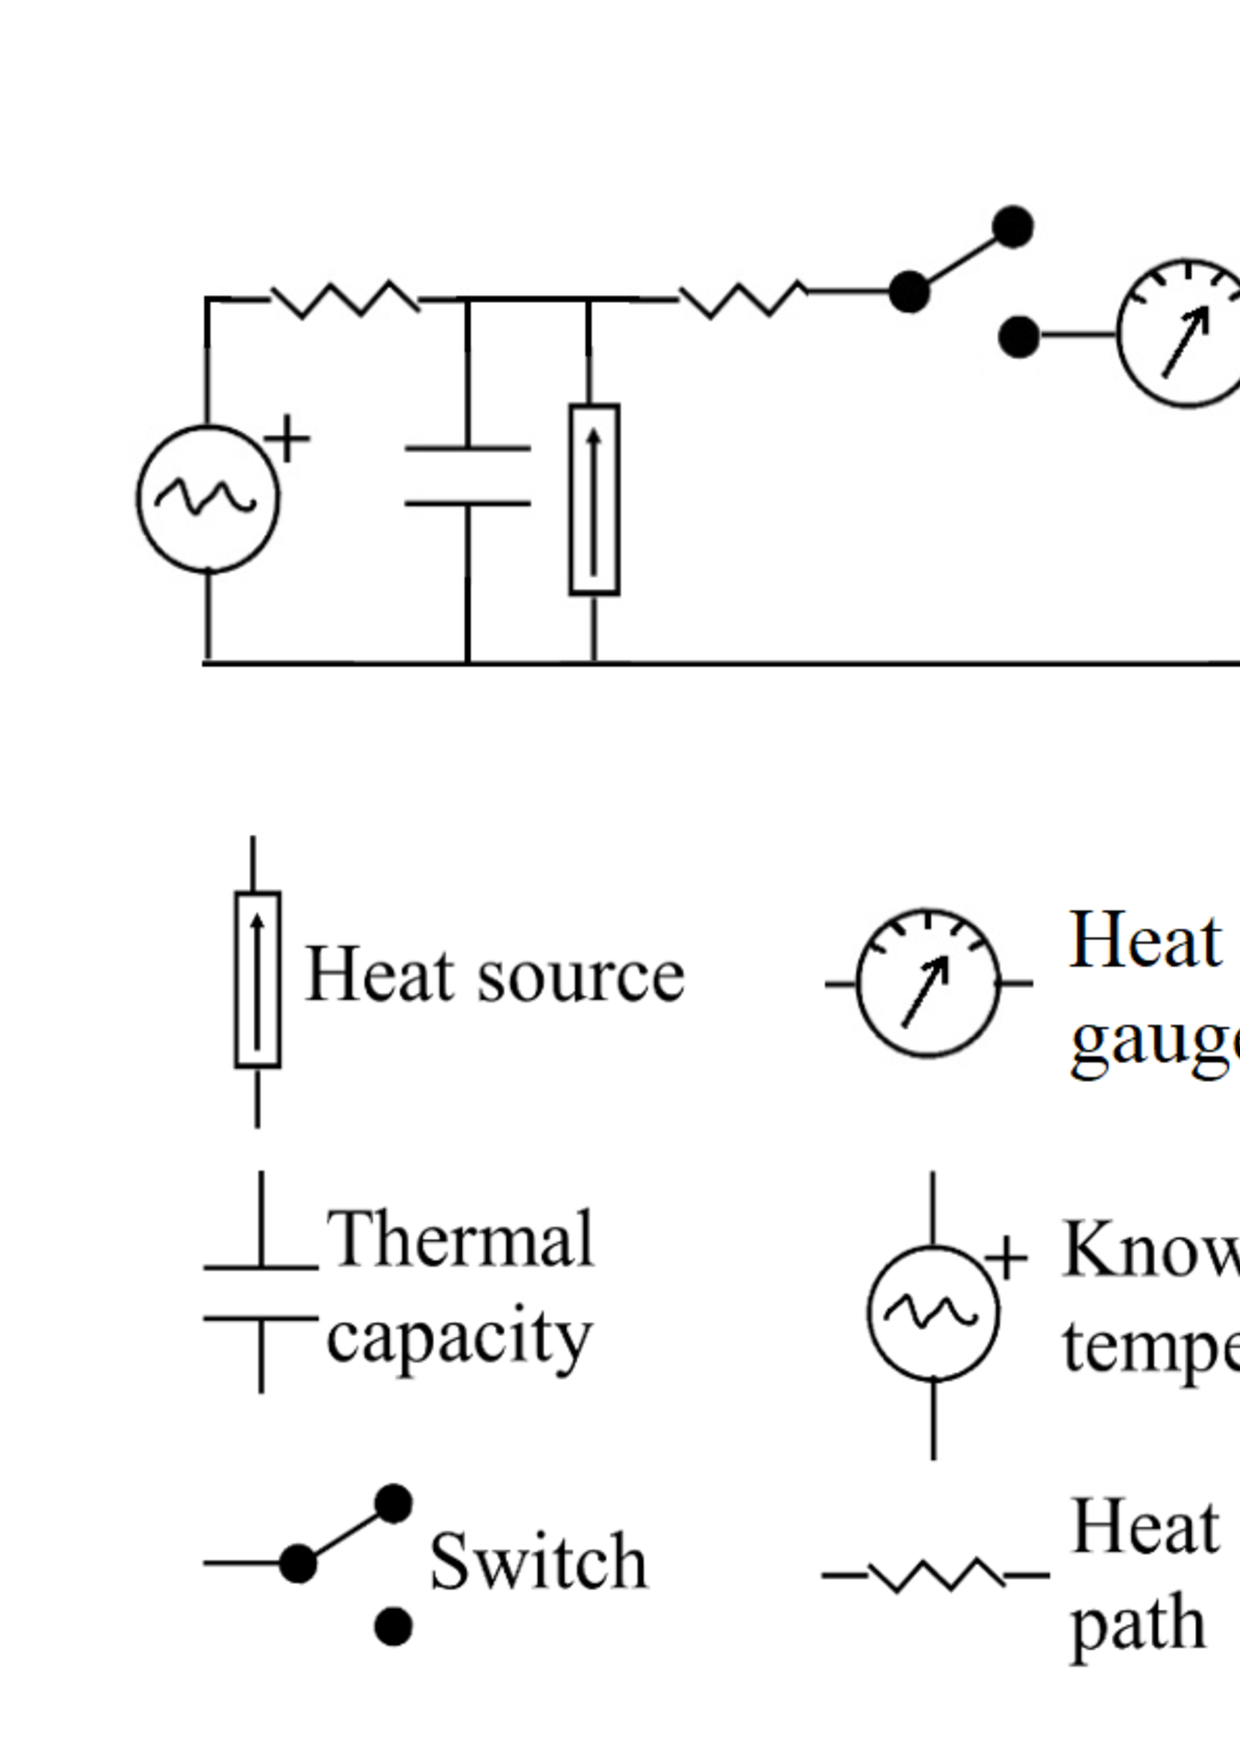
\includegraphics[width=4.5cm,height=4.5cm,keepaspectratio]{./pics/figAlf.pdf}}
\caption{Dual-mode RC network}\vspace*{-6pt}
  \label{fig:alf}
\end{figure}

The conditioning system is governed in our case by a thermostat with a timer that turns it on and off. For this reason one need to consider that the RC-network that represents the building needs to change topologies depending on the operation (on or off). We have considered a dual-mode RC-network as the one shown in Fig. \ref{fig:alf} and previously introduced by Ramallo-Gonz\'alez on \cite{ramalloidentifying}.



\subsection{Black-box baseline models}

Our proposed black-box models are compared with two baseline approaches that are documented in the literature. The first one is a regression-based electricity load model and the second one is a purely machine learning model that uses the inputs uniquely at the same timestamp than the output. 


\subsubsection{Time-of-week-and-temperature (TWT)}

This algorithm was introduced in \cite{mathieu2011quantifying}. We have chosen it because of its high accuracy, low complexity and low computational cost when compared with the results of other state-of-the-art works methods used through a wide number of buildings \cite{granderson2016accuracy}. 

In this work the predicted load is a sum of two terms: a ``time of week effect" that allows each time of the week to have a different predicted load from the others, and a piecewise-continuous effect of temperature. 

The central point of this algorithm is the creation of several coefficients that will be estimated using multiple ordinary least square regression. There will be a coefficient for every ``time of the week". A time of the week is a unique instant of a week (Monday 1AM, Monday 2AM, ad so on). For example, there will br $24 \times 5 = 120$ (24 hours and 5 working days) coefficients in the case of hourly predictions or  $4\times 24 \times 5 = 480$ in the case of 15 minutes prediction. In addition, also some coefficients related to the temperature need to be calculated. Basically, the range of outside temperature data is cut into 6 levels and each of those has an assigned coefficient.

\subsubsection{Gaussian}

A Gaussian process (GP) modelling framework determineing energy savings and uncertainty levels in measurement and verification (EM\&V) practice is presented in \cite{heo2012gaussian}.  In this work they compare a black-box approach to the regular linear regression techniques that are widely explored on the literature and they state that GP models can capture complex nonlinear and multivariable interactions as well as multiresolution trends of energy behaviour thanks to the Bayesian approach under which they are developed. 

\subsection{Model Accuracy Metrics}

To assess model accuracy, this work uses two metrics: the mean absolute percentage of error (MAPE) and the coefficient of variation of the root mean squared error (CVRMSE).
The MAPE metric has been used in a wide number of electricity prediction studies \cite{fan2014development, edwards2012predicting}
. It expresses the average absolute error as a percentage and is calculated as it follows:

\[
 MAPE = \frac{1}{n}\sum_{i=1}^{n} |\frac{y_i-\bar{y_i}}{y_i}|\times 100,
\]

where $y_i$ is the real consumption, $\bar{y_i}$ is the predicted consumption and $n$ is the number of observations.

Also the CVRMSE has often been used in energy prediction studies \cite{quilumba2015using} and will be used also here %26
. It evaluates how much error varies with respect
to the actual consumption mean and is calculated as it follows:

\[
 CVRMSE = \frac{\sqrt{\frac{1}{n-1}\sum_{i=1}^{n}(y_i-\bar{y_i})^2}}{\bar{y}} \times 100,
\]


\subsection{Savings Metrics}

To determine energy savings and uncertainty levels from energy efficiency measures, the IPMVP [13] and ASHRAE’s Guideline 14 [2] provide three methods. The one that is suitable for our approach is whole-building metering, since it compares the total energy demand or cost during pre-experiment and post-experiments periods.

%How to assess the accuracy and usefulness of whole-building energy models by testing predictions of baseline energy use against actual energy use being the objective to quantify and minimize the uncertainty in reported whole-building savings, which depends on baseline model effectiveness, building predictability, and depth of savings being measured \cite{kramer2013energy}.

The predictive baseline models' output is the metered pre-experiment energy use energy$_{pre}$ and uses the so called predictors environmental conditions inputs$_{pre}$ as inputs of the model. The error in reported savings is proportional to the error in the baseline model forecasts.


\section{Use case}

The reference building in which the proposed procedure has been carried out to generate accurate building models is the Chemistry Faculty of the University of Murcia, which is a building used as a pilot for the H2020 project ENTROPY \footnote{http://entropy-project.eu/}.  

The data that is used in order to build and train our baseline cirresponds to 1 year worth of data, from February 2016 to February 2017. 

\begin{figure}[h]%\vspace*{4pt}
\centering
\centerline{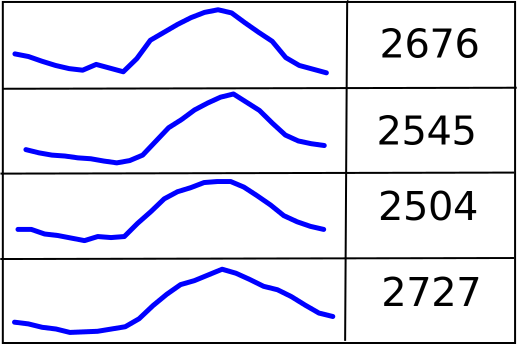
\includegraphics[width=4.5cm,height=4.5cm,keepaspectratio]{./pics/table_inputs_outputs.pdf}}
\caption{Daily temperature time series input and consumption output. Numbers in Watts hour}\vspace*{-6pt}
  \label{fig:inout}
\end{figure}

\subsection{Black-box approach}

Our black-box methodology is highly versatile with respect to the input data i.e.,  it allows the addition of variables with minimal effort. We started them method on a constructive way by relating the 24 temperature values of each day with the energy consumption of the building (see Fig. \ref{fig:inout}).

Having introduced the daily temperature time series, we considered that the addition of a categorical variable indicating season was irrelevant. The subject building has several features that are typical of educational buildings: the load %is temperature-dependent load 
on weekends is substantially lower than the load on weekdays and there are also differences among week days (mainly Fridays).
In those terms, we used analysis of variance (ANOVA) in order to determine whether there exist differences between the consumption of the different days of the week (p-value = 0.001 $<$ 0.05) . 	In a \textbf{post-hoc}  test, the conclusion is that we can consider that Fridays have a different behaviour than the rest of the days of the week, this could be due to lower occupation. With this knowledge, we considered neccesary to add a dychotomus variable that indicates the kind of day of the week. Weekends and holidays consumption is estimated with the mean of the previous weekends and holidays.

The algorithms that we found relevant to use within our black-box methodology are: Support Vector Regression (SVR), Regression Forest (RF) and Extreme Gradient Boosting (XGB). 

SVR works in a similar fashion to Support Vector Machines (SVM). Whereas SVM is a classification technique, SVR fits the optimal curve out of which the training data do not deviate more than a small number $\epsilon$. More specifically, during classification the samples that are close to the margin are penalised even if they are correctly classified, whereas in the regression method an acceptable deviation margin of the samples from the prediction curve is set.
The free parameter of this model is C, the penalty parameter of the error term. C is the weight of how much samples inside the margin cotribute to the overall error.%, and ε, the distance between points predicted and the actual values.



Regression Forest is a type of ensemble learning method, where a group of weak models combine to form a more powerful model. In Regression Forest multiple regression trees are grown. In order to predict a new observation, each tree gives its own prediction and then the average of the output of each one is taken. The algorithm works growing a tree from each random with replacement samples taken from the training. For each node, $m_{try}$ variables are selected at random out of the number of inputs. The best split on these $m_{try}$ is used to split the node. The hyperparameter of Regression Forest that we will search for is the number of random variables that are taken into account on every split: $m_{try}$. 


XGB is built on the principles of gradient boosting and designed for speed and performance (from where it comes the term ``extreme").
Gradient Boosted Regression is a technique that generates a prediction through an ensemble of weak prediction models, decision trees in our case. The concept is to sequentially build the model by fitting a weak prediction model on the weighted training data set, where the higher weights are assigned on samples that were previously difficult to predict.

The free parameters that are adjusted in this model are the maximum depth limit of number of nodes in the tree, the minimum number of samples required to split an internal node and the learning rate by which the contribution of each tree is shrunk.

For the sake of comparison, we are using also the Gaussian Process for modelling the instantaneous consumption prediction using the current input values (mean daily temperature for daily cosumption or mean hourly temperature for hourly consumption).


\subsection{Grey-box approach}

In the case of our grey-box methodology, a topology was selected that could represent the building adequately.


Once the system was defined, an optimisation algorithm was used to find the values that minimise the RMSE (10 minutes intervals) of the simulated power consumption. To ensure that the data was used adequately, the total electricity consumption was separated onto an un-seasonal component and a seasonal one. The un-seasonal component was used as electric loads and the seasonal component was considered as the heating and cooling load. The building is equipped with a boiler and radiators network that contribute to some of the heating loads. To take into account this effect, the prelimiary estimation was done using the summer period. From that, the heating portion that is given by radiators was extracted. This ratio was used in the consecutive calculations.

The optimisation method to find the parameters of the model was the simplex. method. The termination criteria was to get a change on the solution smaller than 0.01 in all parameters. %The calculation took approximately 6 minutes on a i5 Intel computer 2.7 running single threaded.


\subsection{Results}

The prediction metrics are summarised on Table I. The first three methods: SVR, RF, XGB  belong to the group of black-box models and are blind to the physics of the problem. Also we have the TWT the GP and the Grey-box model the later with information about the physical phenomenon on the model topology. As it can be seen, they return the best results compared to the Gaussian method, that is applied in a more traditional way, that is relating the instantaneous consumption measurement with the instantaneous inputs measurements and also with our grey-box model approach. 

Between the three black-box methods, Random Forest is the one that stands out getting a CVRMSE of 9 and 5 \%  and a MAPE of 6, 4.5 \% for the daily and weekly predictions respectively. We have plotted the prediction vs the real daily consumption in Fig. \ref{fig:daily} and weekly in Fig. \ref{fig:weekly} .

\begin{center}
\captionof{table}{Metrics}
\resizebox{\columnwidth}{!}{%
\begin{tabular}{cc|c|c|c|c|c|c|c}
\cline{3-8}
& & \multicolumn{6}{ c| }{Models} \\ \cline{3-8}
& & SVR & \textbf{RF} & XGB & TWT & Gauss & Grey   \\ \cline{1-8}
\multicolumn{1}{ |c  }{\multirow{2}{*}{Daily} } &
\multicolumn{1}{ |c| }{CVRMSE} & 12.4 & \textbf{9} & 11& 14.9  & 17.45 & 33.57      \\ \cline{2-8}
\multicolumn{1}{ |c  }{}                        &
\multicolumn{1}{ |c| }{MAPE} & 7.2 & \textbf{6} & 7.3& 12.3 & 15.01 & 43.02      \\ \cline{1-8}
\multicolumn{1}{ |c  }{\multirow{2}{*}{Weekly} } &
\multicolumn{1}{ |c| }{CVRMSE} & 6.4 & \textbf{5} & 6.2 & 11.1 & 16.3 & 19.53  \\ \cline{2-8}
\multicolumn{1}{ |c  }{}                        &
\multicolumn{1}{ |c| }{MAPE} & 5.2 & \textbf{4.5} & 5.5 & 9.4 & 12.3 & 15.48  \\ \cline{1-8}
\end{tabular}
}
\end{center}




%\begin{figure}[h]%\vspace*{4pt}
%\centering
%\centerline{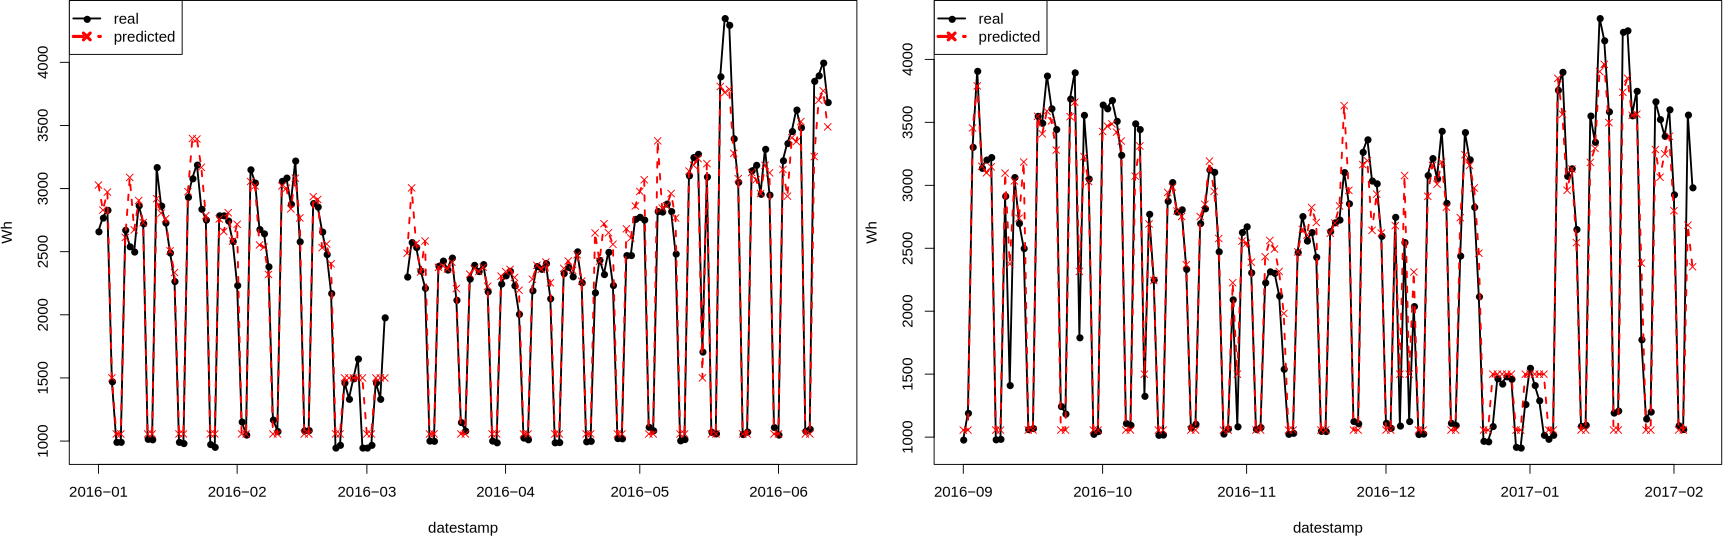
\includegraphics[width=15.5cm,height=15.5cm,keepaspectratio]{./pics/two_daily.pdf}}
%\caption{Daily predictions using RF and real consumption}\vspace*{-6pt}
%  \label{fig:daily}f
%\end{figure}

\begin{figure*}[t!]
  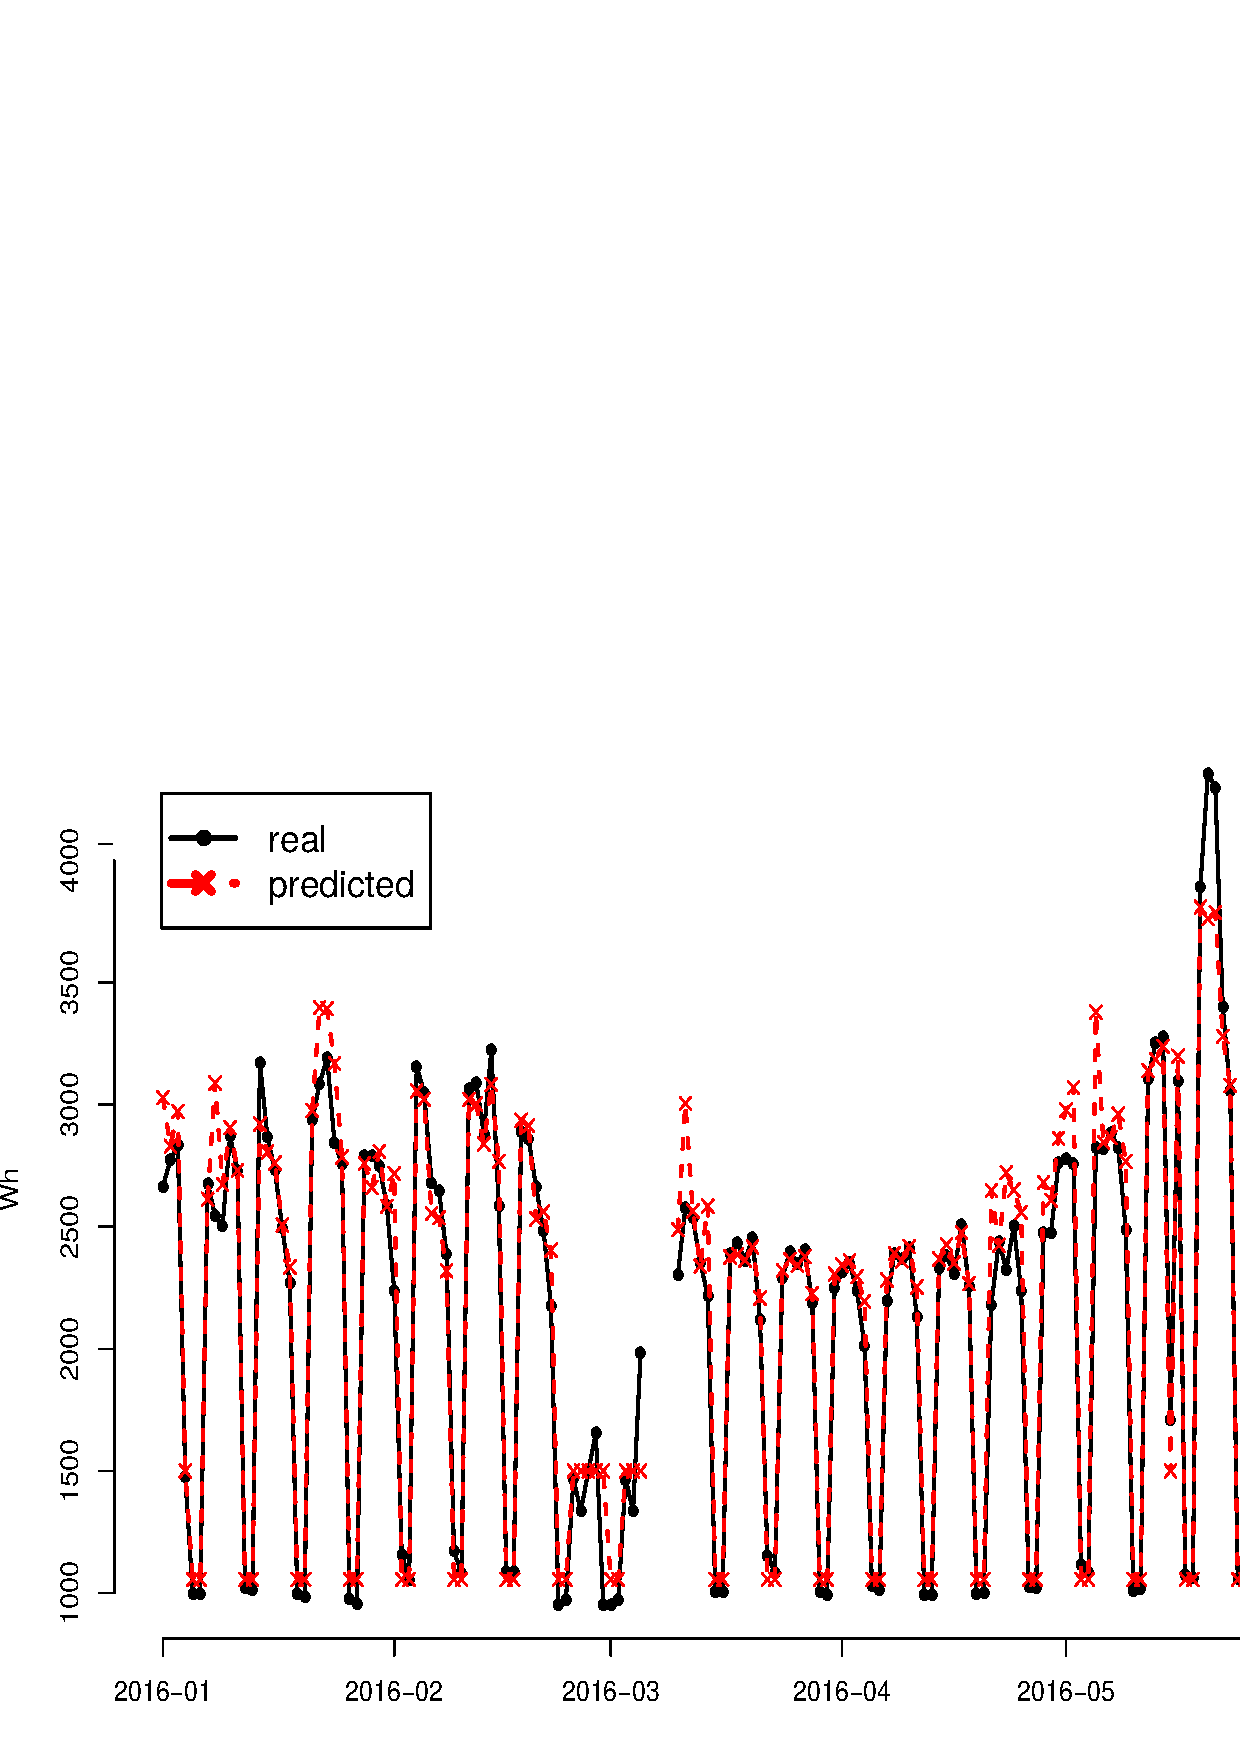
\includegraphics[width=17cm,height=17cm,keepaspectratio]{./pics/two_daily-iii.pdf}
  \caption{Daily predictions using RF and real consumption}
  \label{fig:daily}
\end{figure*}

%\begin{figure}
%\centering
%\begin{subfigure}[b]{0.55\textwidth}
%   \includegraphics[width=8cm,height=5cm]{./pics/daily_RF1.pdf}
%   \caption{}
%   \label{fig:Ng1} 
%\end{subfigure}
%
%\begin{subfigure}[b]{0.55\textwidth}
%   \includegraphics[width=8cm,height=5cm]{./pics/daily_RF2.pdf}
%   \caption{}
%   \label{fig:Ng2}
%\end{subfigure}
%\label{fig:daily}
%\caption[Two numerical solutions]{(a) (b) As for (a) but over a second period of time}
%\end{figure}

\begin{figure*}[t!]\label{fig:weekly}%\vspace*{4pt}
\centering
\centerline{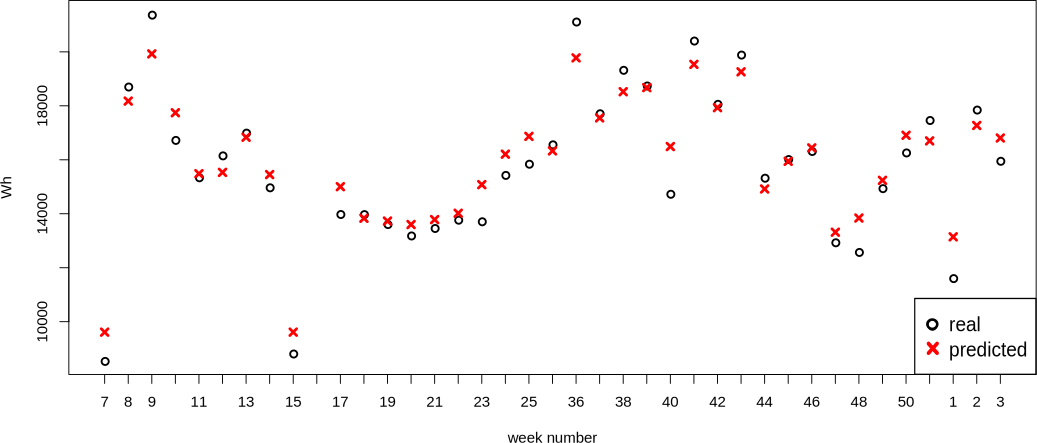
\includegraphics[width=12cm,height=12cm,keepaspectratio]{./pics/weekly.pdf}}
\caption{Weekly predictions using RF and real consumption}\vspace*{-6pt}
  \label{fig:weekly}
\end{figure*}

\section{Discussion}

As previously mentioned, this paper aims to evaluate if the fact that the RC-networks on the grey-box inverse modelling contains basic information about the physical system (i.e. how the thermodynamics of the building should be) deliver any advantage for energy consumption prediction of a smart building for measurement and verification purposes. To this aim, they were compared to our proposed state-of-the-art black-box method in which no prior high level information about the system is included (i.e. they are blind to the physics of the problem) and that combines statistical analysis and machine learning techniques. %For that, the errors and computational times of a grey-box model have been estimated for the case under study.

%This work has introduced two ways for predicting energy consumption for use in applications focused on whole-building measurement and verification for energy efficiency programs.

%One way is purely data-driven, based on statistical analysis and machine learning algoritms, the so called black-box approach. The other way is based on the physical properties of the building and its relationship with the data, that is a grey-box approach.

We have shown that using the daily temperature time series we are able to capture the behaviour of the people better than if instantaneous values are used for predicting consumption (Gaussian) or if we use a barrage of coefficients in linear regression for modelling each small part of the day (TWT). 

This result could in some aspect have been anticipated, energy consumption is a phenomenon heavily dominated by human behaviour. The physics of the building can capture the response of passive elements such as walls and windows, but behavioural patterns are out of their scope.

A drawback of the baseline data-driven models is that they neglect the correlation between timestamps. TWT creates artificial features in order to model each moment independently. We understand the input data as time series and we are considering in an indirect way all the interactions that building and temperature experience towards consumption.
Also, the application of regression techniques have to be preceded by the assessment of the asumptions that have to be fulfilled: normality, little multicollinearity, no auto correlation and homocedasticity. However, a black-box models does not need such assumptions.


That way, we have created a methodology where the combination of time series and current state variables is possible and provides a wide variety of techniques related to time series that can be used to improve the results of the analysis.

\section{Conclusions and future work}

After applying all the baseline models, grey-box approach and black-box approach we have seen that black-box models overcome the rest.

%A very important characteristic of the black-box approach is its generality. Even if we would have obtained similar results with the grey-box models, black-box models are clearly more generalizable than the previous. 


It is foreseen, a future research avenue consists on the application of the same models to several buildings that share some characteristics. That is, they belong to the same environment: different faculties of a university (where students and professors behave similarly among buildings), several houses of a neighbourhood or different comercial buildings of the same city.

Reducing the total time required for EM\&V is key to scaling the deployment of energy efficiency projects in general, and reducing overall costs \cite{granderson2015automated}. That is why a transfer learning approach has to be considered in future studies in order to reduce the quantity of data that needs to be collected for creating a reasonable building model.

Also, a wider study on the way of introducing the time series to the algorithms should be done. That means, applying time series segmentation and representation techniques for finding more representative ways of introducing the data. Or also considering feature selection techniques.


Overall, we believe that the work reported on this paper has explored yet another discipline in which data-driven methods are overweighting traditional methods based on the physics. The results once more demonstrate, that data science can provide an “as good” or “better” answer than physically informed approaches.

\section*{Acknowledgements}

This work has been partially funded by MINECO TIN2014-52099-R project (grant BES-2015-071956) and ERDF funds, by the European Commission through the H2020-ENTROPY-649849 EU Project. Ramallo-González would like to thank CARM via Fundación Séneca for the program Saavedra Fajardo, project number: 20035/SF/16.


% An example of a floating figure using the graphicx package.
% Note that \label must occur AFTER (or within) \caption.
% For figures, \caption should occur after the \includegraphics.
% Note that IEEEtran v1.7 and later has special internal code that
% is designed to preserve the operation of \label within \caption
% even when the captionsoff option is in effect. However, because
% of issues like this, it may be the safest practice to put all your
% \label just after \caption rather than within \caption{}.
%
% Reminder: the "draftcls" or "draftclsnofoot", not "draft", class
% option should be used if it is desired that the figures are to be
% displayed while in draft mode.
%
%\begin{figure}[!t]
%\centering
%\includegraphics[width=2.5in]{myfigure}
% where an .eps filename suffix will be assumed under latex, 
% and a .pdf suffix will be assumed for pdflatex; or what has been declared
% via \DeclareGraphicsExtensions.
%\caption{Simulation Results}
%\label{fig_sim}
%\end{figure}

% Note that IEEE typically puts floats only at the top, even when this
% results in a large percentage of a column being occupied by floats.


% An example of a double column floating figure using two subfigures.
% (The subfig.sty package must be loaded for this to work.)
% The subfigure \label commands are set within each subfloat command, the
% \label for the overall figure must come after \caption.
% \hfil must be used as a separator to get equal spacing.
% The subfigure.sty package works much the same way, except \subfigure is
% used instead of \subfloat.
%
%\begin{figure*}[!t]
%\centerline{\subfloat[Case I]\includegraphics[width=2.5in]{subfigcase1}%
%\label{fig_first_case}}
%\hfil
%\subfloat[Case II]{\includegraphics[width=2.5in]{subfigcase2}%
%\label{fig_second_case}}}
%\caption{Simulation results}
%\label{fig_sim}
%\end{figure*}
%
% Note that often IEEE papers with subfigures do not employ subfigure
% captions (using the optional argument to \subfloat), but instead will
% reference/describe all of them (a), (b), etc., within the main caption.


% An example of a floating table. Note that, for IEEE style tables, the 
% \caption command should come BEFORE the table. Table text will default to
% \footnotesize as IEEE normally uses this smaller font for tables.
% The \label must come after \caption as always.
%
%\begin{table}[!t]
%% increase table row spacing, adjust to taste
%\renewcommand{\arraystretch}{1.3}
% if using array.sty, it might be a good idea to tweak the value of
% \extrarowheight as needed to properly center the text within the cells
%\caption{An Example of a Table}
%\label{table_example}
%\centering
%% Some packages, such as MDW tools, offer better commands for making tables
%% than the plain LaTeX2e tabular which is used here.
%\begin{tabular}{|c||c|}
%\hline
%One & Two\\
%\hline
%Three & Four\\
%\hline
%\end{tabular}
%\end{table}


% Note that IEEE does not put floats in the very first column - or typically
% anywhere on the first page for that matter. Also, in-text middle ("here")
% positioning is not used. Most IEEE journals/conferences use top floats
% exclusively. Note that, LaTeX2e, unlike IEEE journals/conferences, places
% footnotes above bottom floats. This can be corrected via the \fnbelowfloat
% command of the stfloats package.



% trigger a \newpage just before the given reference
% number - used to balance the columns on the last page
% adjust value as needed - may need to be readjusted if
% the document is modified later
%\IEEEtriggeratref{8}
% The "triggered" command can be changed if desired:
%\IEEEtriggercmd{\enlargethispage{-5in}}

% references section

% can use a bibliography generated by BibTeX as a .bbl file
% BibTeX documentation can be easily obtained at:
% http://www.ctan.org/tex-archive/biblio/bibtex/contrib/doc/
% The IEEEtran BibTeX style support page is at:
% http://www.michaelshell.org/tex/ieeetran/bibtex/
\bibliographystyle{IEEEtran}
% argument is your BibTeX string definitions and bibliography database(s)
\bibliography{IEEEabrv,bib.bib}
%
% <OR> manually copy in the resultant .bbl file
% set second argument of \begin to the number of references
% (used to reserve space for the reference number labels box)
%\begin{thebibliography}{1}

%

%\end{thebibliography}




% that's all folks
\end{document}


